\documentclass[conference]{IEEEtran}
\usepackage{cite}
\usepackage{amsmath,amssymb,amsfonts}
\usepackage{graphicx}
\usepackage{textcomp}
\usepackage{xcolor}
\usepackage{pgfplots}
\usepackage{pgfplotstable}
\usepackage{booktabs}
\usepackage{url}
\pgfplotsset{compat=1.18}

\usepgfplotslibrary{groupplots}

\begin{document}

\title{Geographic Address Assignment Optimization\\for Emergency Services Workers}

\author{\IEEEauthorblockN{Bob Iannucci}
\IEEEauthorblockA{Carnegie Mellon University, Silicon Valley\\
Moffett Field, CA 94035\\
bob@rail.com}}

\maketitle

\begin{abstract}
During disaster response, Emergency Services Workers (ESWs) must visit assigned addresses to assess damage. Minimizing each worker's travel distance while maintaining balanced workloads is critical for rapid response. We formalize this as a balanced geographic partitioning problem over road-network segments --- uninterrupted stretches of roadway between intersections --- with walking distances constrained to the street network. Each segment carries a precomputed $4 \times 4$ cost matrix that captures all traversal options (through-walk, out-and-back, zigzag, U-turn) as a function of entry/exit port and address distribution. We evaluate three partitioning strategies across 41 neighborhoods in Palo Alto, California (52--5,101 addresses). No single algorithm dominates; the winner depends on neighborhood geometry. The cost matrix formulation subsumes the U-turn optimization (33--71\% walk reduction) as an emergent property rather than a separate heuristic. We recommend an oracle approach: run all strategies, score each, select the best. The combined algorithm runs in under one second, enabling real-time assignment during emergency operations.
\end{abstract}

\begin{IEEEkeywords}
disaster response, geographic partitioning, vehicle routing, emergency services, address assignment, road network, heuristic algorithms
\end{IEEEkeywords}

\section{Introduction}

Post-disaster damage assessment requires Emergency Services Workers (ESWs) to physically visit assigned addresses, inspect structures, and report conditions via mobile devices. The speed of this process directly affects emergency response effectiveness: faster assessment means faster resource allocation to the most critical areas~\cite{fema2023}.

In the ES-Link system~\cite{eslink}, a Neighborhood Preparedness Coordinator (NPC) assigns addresses to ESWs through a web-based map interface. Manual assignment is tedious and does not optimize for worker travel distance. We developed an auto-assignment feature that distributes addresses across $N$ workers, minimizing travel distance while maintaining balanced workloads.

The problem combines elements of the Capacitated Vehicle Routing Problem (CVRP)~\cite{toth2014} and balanced graph partitioning~\cite{andreev2006}. Unlike classical VRP, our ``vehicles'' (ESWs on foot) start from arbitrary positions, there is no depot, and the primary constraint is workload balance rather than vehicle capacity. The general problem is NP-hard~\cite{garey1979}, so we seek practical heuristics that produce good solutions in real-time.

\subsection{Contributions}

\begin{itemize}
\item A road-network segment model that decomposes streets into atomic walkable units between intersections, with addresses snapped to segments and classified by side
\item A $4 \times 4$ cost matrix per segment that captures all traversal options (through-walk, out-and-back, zigzag, U-turn) as a function of entry/exit port, street width, and address distribution --- subsuming the split/merge decision automatically
\item Street-constrained walking distances that prohibit jumping between non-adjacent addresses
\item Three partitioning strategies (bisect, NN chain, right-hand chain) operating on segments with port-aware chaining
\item Empirical evaluation across 41 real neighborhoods with training/test validation
\item Simulated annealing analysis showing that the foothill problem is real but bounded
\item Evidence that no single algorithm dominates and the oracle approach is optimal
\end{itemize}

\section{Problem Formulation}

\subsection{Road Network Model}

We model the street network as a graph $G = (V, E)$ extracted from OpenStreetMap data, where vertices $V$ are \emph{intersections} (nodes where two or more road ways meet, or way endpoints) and edges $E$ are \emph{road segments} --- uninterrupted stretches of roadway between intersections. Within a segment, no turns are possible; turns occur only at segment endpoints.

\begin{description}
\item[Segment] A maximal chain of road edges between intersection nodes, with street name, road class, polyline geometry, and length $D$.
\item[Sub-segment] One side of a segment. Each segment yields up to two sub-segments (left side, right side), determined by which side of the road's centerline each address falls on. A sub-segment contains addresses $a_1, a_2, \ldots, a_n$ ordered by their fractional position $t_i \in [0,1]$ along the segment ($t=0$ at the start intersection $S$, $t=1$ at the end intersection $E$).
\end{description}

ESWs are constrained to walk along streets at all times. They may walk house-to-house within a sub-segment, turn a corner at an intersection, or cross a street (U-turn), but may not jump over houses or pass through properties.

\subsection{Segment Traversal Cost}

Each segment endpoint has two \emph{ports} --- one per sidewalk --- giving four ports per segment: $S_L, S_R, E_L, E_R$. An ESW enters at one port and exits at another. The minimum traversal cost depends on which ports are used and the distribution of addresses on each side.

Within a segment, the ESW proceeds monotonically (never backtracks), crossing the street as needed to reach addresses on the opposite side. Backtracking is always dominated by crossing when the street width $w$ is less than twice the along-street gap between consecutive addresses --- which holds for virtually all residential streets.

Addresses sorted by position form \emph{runs} --- maximal consecutive groups on the same side. Let $r$ be the number of runs. The cost for a through-traversal entering on side $s$ and exiting on side $e$ is:

\begin{equation}
C(S_s, E_e) = D + k(s, e) \cdot w
\label{eq:through-cost}
\end{equation}

where $k(s,e) = (r-1) + [s \neq \text{side of first run}] + [e \neq \text{side of last run}]$ counts the mandatory side-changes plus entry/exit adjustments. The Iverson brackets are 0 or 1.

For out-and-back traversals, the return leg carries no addresses, so zero crossings on return:

\begin{equation}
C(S_s, S_e) = 2 \cdot t_n \cdot D + k_{\text{out}}(s) \cdot w
\label{eq:outback-cost}
\end{equation}

The exit side $e$ is free on the return --- the ESW walks back on whichever sidewalk connects best to the next segment.

The full $4 \times 4$ cost matrix for each segment is precomputed in $O(n)$ time from the address sequence. This formulation subsumes the split/merge decision automatically:

\begin{itemize}
\item \textbf{Dense alternating addresses} ($r$ large): Through-traversal cost $D + r \cdot w$ becomes expensive. The optimizer routes the ESW down one side ($S_L \to E_L$, cost $D$), crosses once at $E$, and assigns the return side as a separate traversal --- the U-turn pattern emerges from the cost matrix without explicit sub-segment splitting.
\item \textbf{Addresses grouped by side} ($r$ small): Through-traversal at $D + k \cdot w$ is cheap. The zigzag pattern is optimal.
\item \textbf{Single-sided segment} ($r = 1$): Zero crossings. The matrix reduces to the four cases $\{D, D, 2t_n D, 2(1-t_1)D\}$.
\item \textbf{Cul-de-sac} ($S = E$): Ports collapse to $\{S_L, S_R\}$. All traversals are out-and-back.
\end{itemize}

\subsection{Objective}

Given $M$ segments (each with a precomputed $4 \times 4$ cost matrix) and $N$ ESWs, find a partition $\{P_1, P_2, \ldots, P_N\}$ of the segments, an ordering within each partition, and port choices for each segment, that minimize:

\begin{equation}
\max_{k \in \{1..N\}} W(P_k)
\end{equation}

where the total walk distance for ESW $k$ is:

\begin{equation}
W(P_k) = \underbrace{\sum_{i=1}^{|P_k|} C(\text{in}_i, \text{out}_i)}_{\text{productive (within-segment)}} + \underbrace{\sum_{i=1}^{|P_k|-1} d_{\text{road}}(\text{out}_i, \text{in}_{i+1})}_{\text{unproductive (between-segment)}}
\label{eq:total-walk}
\end{equation}

The first sum is \emph{productive} walking (visiting addresses within segments). The second sum is \emph{unproductive} walking (traveling between segments along the road network). A good assignment minimizes unproductive walking while balancing the total.

The balance constraint requires:
\begin{equation}
\frac{\max_k |P_k|}{\min_k |P_k|} \leq \beta
\end{equation}
where $|P_k|$ is the total number of addresses in ESW $k$'s assigned segments and $\beta \approx 1.0$.

\subsection{Data Sources}

Segments are derived from the OpenStreetMap road network, imported via \texttt{osm2pgsql} from a Geofabrik California PBF extract (1.3\,GB), filtered to the Palo Alto bounding box ($37.35$--$37.48^\circ$N, $122.05$--$122.20^\circ$W). Road types included: motorway through living\_street. Intersections are identified as nodes appearing in more than one OSM way or at way endpoints.

Addresses come from the City of Palo Alto municipal address database (44,115 addresses), stored in PostGIS with WGS84 coordinates. Each address is snapped to its nearest road segment (within 200\,m) and classified as left or right side by the cross-product of the road direction vector and the address displacement vector. The per-segment cost matrix is then computed from the address positions and sides.

Inter-segment distances $d_{\text{road}}$ are computed as shortest paths on the road network graph using Dijkstra's algorithm between intersection nodes. For each pair of adjacent segments sharing an intersection, the transition cost is the road-network distance between their respective ports (zero for ports at the same intersection, street-crossing width $w$ for ports on opposite sidewalks of the same intersection).

\section{Algorithms}

All algorithms operate on the segment graph: segments are nodes with four ports ($S_L, S_R, E_L, E_R$) and precomputed cost matrices; edges between segments carry road-network distances between shared intersections. The algorithms differ in how they order and partition segments across ESWs.

\subsection{Single-Worker Baseline}

To establish a lower bound, we compute the walk distance for a single ESW visiting all segments using nearest-neighbor construction on segment ports:

\begin{enumerate}
\item Start at an arbitrary segment, entering at the cheapest port
\item Traverse the segment (cost from the cost matrix)
\item From the exit port, find the unvisited segment whose nearest port minimizes the road-network transition distance
\item Enter that segment at the chosen port, traverse it
\item Repeat until all segments are visited
\end{enumerate}

The theoretical ideal for $N$ workers is $W_{baseline} / N$, though this is unachievable in practice due to the overhead of inter-partition transitions.

\subsection{Strategy A: Nearest-Neighbor Chain Slicing}

Chain all segments using the port-to-port nearest-neighbor heuristic (as in the baseline), then partition the chain into $N$ contiguous groups at the target address count boundary $\lceil |A|/N \rceil$. We try all possible starting segments and keep the best result.

\textbf{Advantages:} Perfect count balance ($\beta = 1.00$). Segments remain in walk order within each partition.

\textbf{Disadvantages:} Cut points are determined solely by count, not geographic boundaries. A chain that snakes through the neighborhood may produce partitions that are geographically scattered.

\subsection{Strategy B: Right-Hand-Rule Chain Slicing}

A variant of Strategy~A that uses the ``wall follower'' heuristic instead of pure nearest-neighbor. After exiting a segment, the next segment is chosen by minimizing a score that combines road-network distance with clockwise turn angle from the current heading:

\begin{equation}
\text{score}(s) = d_{\text{road}}(\text{exit}, \text{entry}_s) + 0.5 \cdot \theta_{\text{clockwise}}
\end{equation}

where $\theta_{\text{clockwise}}$ is the clockwise angular difference between the current heading and the bearing to the candidate segment's entry port. This creates a spiral traversal pattern that naturally covers contiguous areas, particularly effective on circular street layouts (Fig.~\ref{fig:rh-path}).

\textbf{Advantages:} Spiral pattern avoids backtracking on curved/circular streets.

\textbf{Disadvantages:} May produce suboptimal chains on regular grids where straight-line traversal is better.

\subsection{Strategy C: Recursive Geographic Bisection}

Recursively split the segment set along the longer geographic axis (latitude or longitude), using segment centroids for sorting:

\begin{enumerate}
\item Determine whether the latitude or longitude range is larger
\item Sort segments by centroid along the longer axis
\item Split at position $\lfloor M \cdot \lceil N/2 \rceil / N \rfloor$
\item Recurse on each half with $\lceil N/2 \rceil$ and $\lfloor N/2 \rfloor$ workers
\item Re-order each final partition using port-aware nearest-neighbor chaining
\end{enumerate}

\textbf{Advantages:} Geographic contiguity (each partition is a compact rectangular region), low unproductive walking.

\textbf{Disadvantages:} Cuts are axis-aligned, which may split a segment's natural neighborhood.

\subsection{Intra-Segment Traversal}

Within each segment, the traversal strategy is determined by the cost matrix (Section~II-B). The zig-zag pattern (crossing the street at each address pair) and the U-turn pattern (walking one side then returning on the other) are not separate algorithm choices --- they emerge from the matrix as a function of the number of address runs $r$ and the street width $w$.

Fig.~\ref{fig:uturn-path} illustrates the two extremes on a single street. When $r$ is large (addresses alternate frequently between sides), through-traversal incurs many crossings and the U-turn is cheaper. When $r$ is small (addresses grouped by side), through-traversal with few crossings dominates.

\begin{figure}[htbp]
\centering
\begin{tikzpicture}
\begin{groupplot}[
    group style={group size=2 by 1, horizontal sep=0.6cm},
    width=0.48\columnwidth,
    height=0.45\columnwidth,
    xlabel={Longitude},
    ylabel={Latitude},
    tick label style={font=\tiny},
    label style={font=\small},
    title style={font=\small\bfseries},
]
\nextgroupplot[title={Zig-Zag ($r$ large)}]
\addplot[blue, thick, opacity=0.6] table[x=lon,y=lat] {data/street-zigzag.dat};
\addplot[only marks, mark=*, mark size=1pt, black] table[x=lon,y=lat] {data/street-points.dat};

\nextgroupplot[title={U-Turn ($r$ large, better)}]
\addplot[red, thick, opacity=0.6] table[x=lon,y=lat] {data/street-uturn.dat};
\addplot[only marks, mark=*, mark size=1pt, black] table[x=lon,y=lat] {data/street-points.dat};
\end{groupplot}
\end{tikzpicture}
\caption{Roosevelt Circle (71 addresses): When addresses alternate between sides ($r$ large), zig-zag through-traversal (left) crosses the street at every pair. The U-turn pattern (right) --- walk one side, return on the other --- reduces walk distance by 81\%. The cost matrix selects the cheaper option automatically.}
\label{fig:uturn-path}
\end{figure}

\begin{figure}[htbp]
\centering
\begin{tikzpicture}
\begin{groupplot}[
    group style={group size=2 by 1, horizontal sep=0.6cm},
    width=0.48\columnwidth,
    height=0.45\columnwidth,
    xlabel={Longitude},
    ylabel={Latitude},
    tick label style={font=\tiny},
    label style={font=\small},
    title style={font=\small\bfseries},
]
\nextgroupplot[title={Nearest-Neighbor Chain}]
\addplot[only marks, mark=*, mark size=0.5pt, gray!50] table[x=lon,y=lat] {data/fm-all-points.dat};
\addplot[blue, thick, opacity=0.7, -stealth] table[x=lon,y=lat] {data/fm-nn-path.dat};

\nextgroupplot[title={Right-Hand Rule Chain}]
\addplot[only marks, mark=*, mark size=0.5pt, gray!50] table[x=lon,y=lat] {data/fm-all-points.dat};
\addplot[red, thick, opacity=0.7, -stealth] table[x=lon,y=lat] {data/fm-rh-path.dat};
\end{groupplot}
\end{tikzpicture}
\caption{Fairmeadow segment-level traversal order (connecting segment centroids). Left: Nearest-neighbor jumps to the closest unvisited segment. Right: Right-hand rule prefers clockwise turns, producing a more spiral-like traversal of the circular streets.}
\label{fig:rh-path}
\end{figure}

\subsection{Scoring Function}

All candidate assignments are evaluated by a combined score:

\begin{equation}
\text{Score} = 2 \cdot W_{max} + W_{total} + 5000 \cdot \frac{\sum_k ||P_k| - |A|/N|}{|A|/N}
\end{equation}

where $W_{max} = \max_k W(P_k)$ is the maximum walk distance (fairness, Eq.~\ref{eq:total-walk}), $W_{total} = \sum_k W(P_k)$ is total walk distance (efficiency), and the third term penalizes count imbalance. The winner is the candidate with the lowest score.

\section{Experimental Setup}

\subsection{Data}

We use the City of Palo Alto municipal address database containing 44,115 addresses across 53 neighborhoods, with road-network segments derived from OpenStreetMap. Three neighborhoods with different characteristics were selected:

\begin{table}[htbp]
\caption{Test Neighborhoods}
\begin{center}
\begin{tabular}{lccl}
\toprule
\textbf{Neighborhood} & \textbf{Addresses} & \textbf{Segments} & \textbf{Character} \\
\midrule
Fairmeadow & 307 & TBD & Circular cul-de-sacs \\
Crescent Park & 1,476 & TBD & Rectilinear grid \\
Midtown & 5,101 & TBD & Large rectilinear grid \\
\bottomrule
\end{tabular}
\end{center}
\end{table}

\subsection{Baselines}

Single-ESW nearest-neighbor walk distances establish the theoretical minimum per worker:

\begin{table}[htbp]
\caption{Single-Worker Baselines}
\begin{center}
\begin{tabular}{lccc}
\toprule
\textbf{Neighborhood} & \textbf{NN Walk} & \textbf{Ideal (N=3)} & \textbf{Ideal (N=5)} \\
\midrule
Fairmeadow & 6,677\,m & 2,226\,m & 1,335\,m \\
Crescent Park & 38,652\,m & 12,884\,m & 7,730\,m \\
Midtown & 101,834\,m & 33,945\,m & 20,367\,m \\
\bottomrule
\end{tabular}
\end{center}
\end{table}

\section{Results}

\subsection{Fairmeadow (N=3)}

\begin{figure}[htbp]
\centering
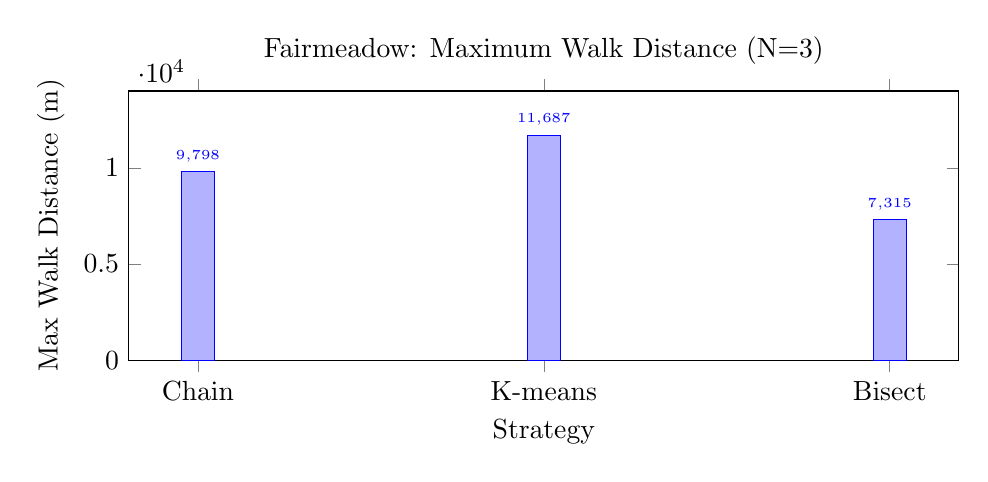
\begin{tikzpicture}
\begin{axis}[
    ybar,
    bar width=12pt,
    xlabel={Strategy},
    ylabel={Max Walk Distance (m)},
    symbolic x coords={Chain, K-means, Bisect},
    xtick=data,
    ymin=0, ymax=14000,
    nodes near coords,
    nodes near coords align={vertical},
    width=\columnwidth,
    height=5cm,
    title={Fairmeadow: Maximum Walk Distance (N=3)},
    every node near coord/.append style={font=\tiny},
]
\addplot coordinates {(Chain,9798) (K-means,11687) (Bisect,7315)};
\end{axis}
\end{tikzpicture}

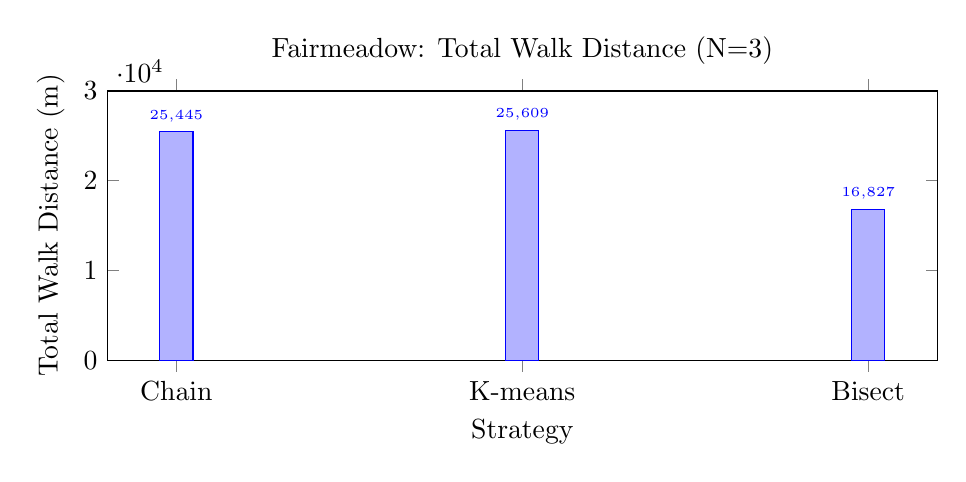
\begin{tikzpicture}
\begin{axis}[
    ybar,
    bar width=12pt,
    xlabel={Strategy},
    ylabel={Total Walk Distance (m)},
    symbolic x coords={Chain, K-means, Bisect},
    xtick=data,
    ymin=0, ymax=30000,
    nodes near coords,
    nodes near coords align={vertical},
    width=\columnwidth,
    height=5cm,
    title={Fairmeadow: Total Walk Distance (N=3)},
    every node near coord/.append style={font=\tiny},
]
\addplot coordinates {(Chain,25445) (K-means,25609) (Bisect,16827)};
\end{axis}
\end{tikzpicture}
\caption{Fairmeadow results. Bisect achieves 34\% lower total walk distance and 25\% lower max walk distance than the best chain slicing variant.}
\label{fig:fairmeadow}
\end{figure}

Bisect wins decisively on Fairmeadow's circular street layout, producing the lowest max walk distance (7,315\,m vs.\ ideal 2,226\,m, 3.3$\times$ overhead) and lowest total walk distance.

\subsection{Crescent Park (N=3)}

\begin{figure}[htbp]
\centering
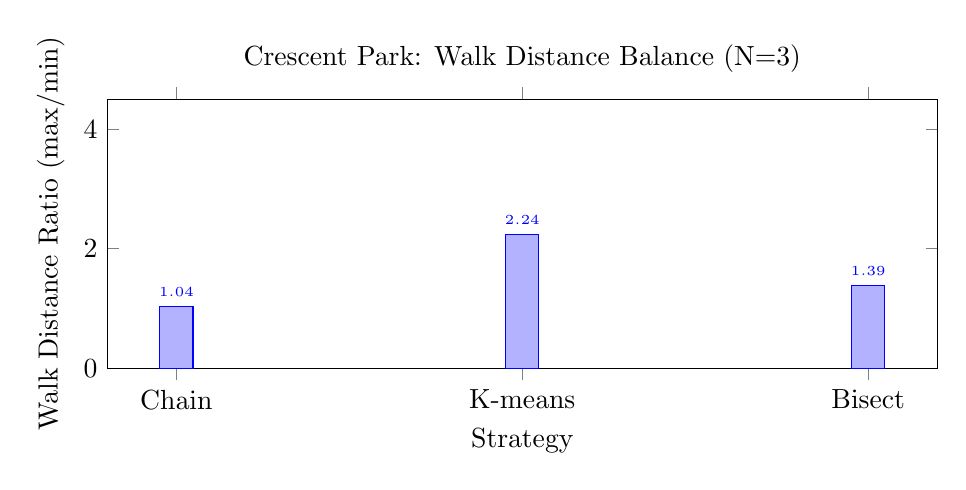
\begin{tikzpicture}
\begin{axis}[
    ybar,
    bar width=12pt,
    xlabel={Strategy},
    ylabel={Walk Distance Ratio (max/min)},
    symbolic x coords={Chain, K-means, Bisect},
    xtick=data,
    ymin=0, ymax=4.5,
    nodes near coords,
    nodes near coords align={vertical},
    width=\columnwidth,
    height=5cm,
    title={Crescent Park: Walk Distance Balance (N=3)},
    every node near coord/.append style={font=\tiny},
]
\addplot coordinates {(Chain,1.04) (K-means,2.24) (Bisect,1.39)};
\end{axis}
\end{tikzpicture}
\caption{Crescent Park walk distance ratios. Chain slicing achieves nearly perfect walk balance (1.04) on this rectilinear grid.}
\label{fig:crescent}
\end{figure}

Chain slicing produced the best walk distance balance (ratio 1.04) on Crescent Park's rectilinear grid. Bisect had lower total walk distance but higher max walk.

\subsection{Midtown (N=3 and N=5)}

\begin{figure}[htbp]
\centering
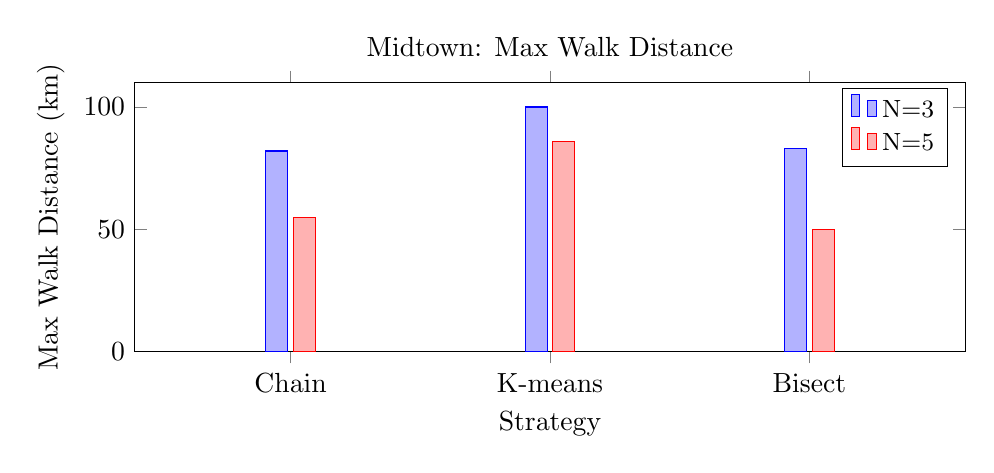
\begin{tikzpicture}
\begin{axis}[
    ybar,
    bar width=8pt,
    xlabel={Strategy},
    ylabel={Max Walk Distance (km)},
    symbolic x coords={Chain, K-means, Bisect},
    xtick=data,
    ymin=0, ymax=110,
    width=\columnwidth,
    height=5cm,
    title={Midtown: Max Walk Distance},
    legend style={at={(0.98,0.98)},anchor=north east,font=\small},
    enlarge x limits=0.3,
]
\addplot coordinates {(Chain,82) (K-means,100) (Bisect,83)};
\addplot coordinates {(Chain,55) (K-means,86) (Bisect,50)};
\legend{N=3, N=5}
\end{axis}
\end{tikzpicture}
\caption{Midtown max walk distances (km) for N=3 and N=5. K-means degrades severely with more workers. Bisect scales well.}
\label{fig:midtown}
\end{figure}

\begin{figure}[htbp]
\centering
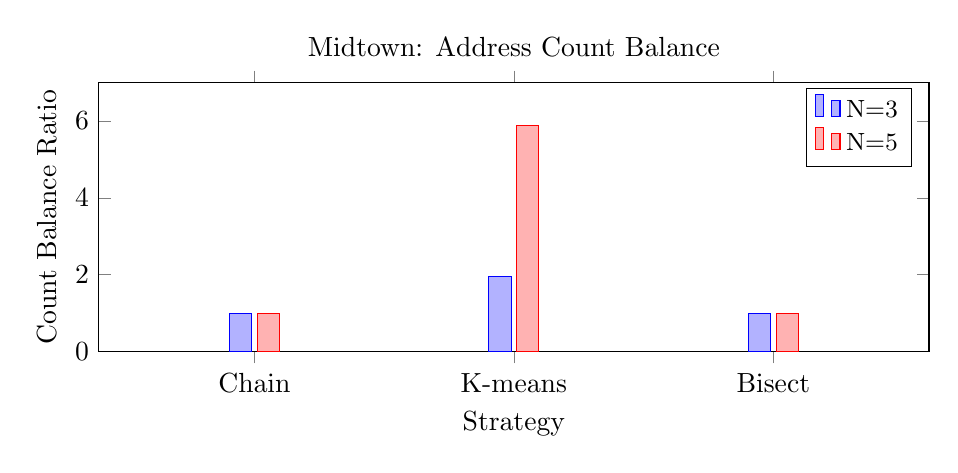
\begin{tikzpicture}
\begin{axis}[
    ybar,
    bar width=8pt,
    xlabel={Strategy},
    ylabel={Count Balance Ratio},
    symbolic x coords={Chain, K-means, Bisect},
    xtick=data,
    ymin=0, ymax=7,
    width=\columnwidth,
    height=5cm,
    title={Midtown: Address Count Balance},
    legend style={at={(0.98,0.98)},anchor=north east,font=\small},
    enlarge x limits=0.3,
]
\addplot coordinates {(Chain,1.00) (K-means,1.96) (Bisect,1.00)};
\addplot coordinates {(Chain,1.00) (K-means,5.88) (Bisect,1.00)};
\legend{N=3, N=5}
\end{axis}
\end{tikzpicture}
\caption{Address count balance. K-means produces severely unbalanced assignments with N=5 (ratio 5.88:1). Chain slicing and Bisect maintain perfect balance.}
\label{fig:balance}
\end{figure}

At $N=5$, k-means assigned 1,735 addresses to one worker and only 295 to another (ratio 5.88:1). Bisect maintained perfect balance while achieving the lowest max walk distance.

\subsection{Walking Trail Visualization}

Fig.~\ref{fig:trails-fm} shows the walking trails for each ESW in Fairmeadow (N=3, ChainNN winner). Blue lines show productive walking (within-segment traversal), red lines show unproductive walking (inter-segment transitions along the road network). Each map shows one ESW's complete route.

\begin{figure*}[htbp]
\centering
\begin{tikzpicture}
\begin{groupplot}[
    group style={group size=3 by 1, horizontal sep=0.8cm},
    width=0.36\textwidth,
    height=0.3\textwidth,
    xlabel={Longitude},
    ylabel={Latitude},
    tick label style={font=\tiny},
    label style={font=\small},
    title style={font=\small\bfseries},
]
\nextgroupplot[title={ESW 1 (18 segments)}]
\addplot[only marks, mark=*, mark size=0.3pt, gray!30] table[x=lon,y=lat] {data/fairmeadow-all-addrs.dat};
\addplot[blue, thick, opacity=0.7] table[x=lon,y=lat] {data/fairmeadow-esw0-segments.dat};
\addplot[red, thick, opacity=0.5, dashed] table[x=lon,y=lat] {data/fairmeadow-esw0-transitions.dat};

\nextgroupplot[title={ESW 2 (19 segments)}]
\addplot[only marks, mark=*, mark size=0.3pt, gray!30] table[x=lon,y=lat] {data/fairmeadow-all-addrs.dat};
\addplot[blue, thick, opacity=0.7] table[x=lon,y=lat] {data/fairmeadow-esw1-segments.dat};
\addplot[red, thick, opacity=0.5, dashed] table[x=lon,y=lat] {data/fairmeadow-esw1-transitions.dat};

\nextgroupplot[title={ESW 3 (6 segments)}]
\addplot[only marks, mark=*, mark size=0.3pt, gray!30] table[x=lon,y=lat] {data/fairmeadow-all-addrs.dat};
\addplot[blue, thick, opacity=0.7] table[x=lon,y=lat] {data/fairmeadow-esw2-segments.dat};
\addplot[red, thick, opacity=0.5, dashed] table[x=lon,y=lat] {data/fairmeadow-esw2-transitions.dat};
\end{groupplot}
\end{tikzpicture}
\caption{Fairmeadow (307 addresses, N=3, ChainNN): Walking trails for each ESW. Blue = productive walking (within-segment traversal). Red dashed = unproductive walking (inter-segment transitions). Gray dots = all addresses in the neighborhood.}
\label{fig:trails-fm}
\end{figure*}

\begin{figure*}[htbp]
\centering
\begin{tikzpicture}
\begin{groupplot}[
    group style={group size=3 by 1, horizontal sep=0.8cm},
    width=0.36\textwidth,
    height=0.3\textwidth,
    xlabel={Longitude},
    ylabel={Latitude},
    tick label style={font=\tiny},
    label style={font=\small},
    title style={font=\small\bfseries},
]
\nextgroupplot[title={ESW 1 (88 segments)}]
\addplot[only marks, mark=*, mark size=0.2pt, gray!30] table[x=lon,y=lat] {data/crescentpark-all-addrs.dat};
\addplot[blue, thick, opacity=0.6] table[x=lon,y=lat] {data/crescentpark-esw0-segments.dat};
\addplot[red, thick, opacity=0.4, dashed] table[x=lon,y=lat] {data/crescentpark-esw0-transitions.dat};

\nextgroupplot[title={ESW 2 (93 segments)}]
\addplot[only marks, mark=*, mark size=0.2pt, gray!30] table[x=lon,y=lat] {data/crescentpark-all-addrs.dat};
\addplot[blue, thick, opacity=0.6] table[x=lon,y=lat] {data/crescentpark-esw1-segments.dat};
\addplot[red, thick, opacity=0.4, dashed] table[x=lon,y=lat] {data/crescentpark-esw1-transitions.dat};

\nextgroupplot[title={ESW 3 (75 segments)}]
\addplot[only marks, mark=*, mark size=0.2pt, gray!30] table[x=lon,y=lat] {data/crescentpark-all-addrs.dat};
\addplot[blue, thick, opacity=0.6] table[x=lon,y=lat] {data/crescentpark-esw2-segments.dat};
\addplot[red, thick, opacity=0.4, dashed] table[x=lon,y=lat] {data/crescentpark-esw2-transitions.dat};
\end{groupplot}
\end{tikzpicture}
\caption{Crescent Park (1,476 addresses, N=3, ChainRH): Walking trails for each ESW on a rectilinear grid. The right-hand rule produces geographically contiguous assignments with minimal red (unproductive) transitions.}
\label{fig:trails-cp}
\end{figure*}

\subsection{Efficiency Analysis}

\begin{figure}[htbp]
\centering
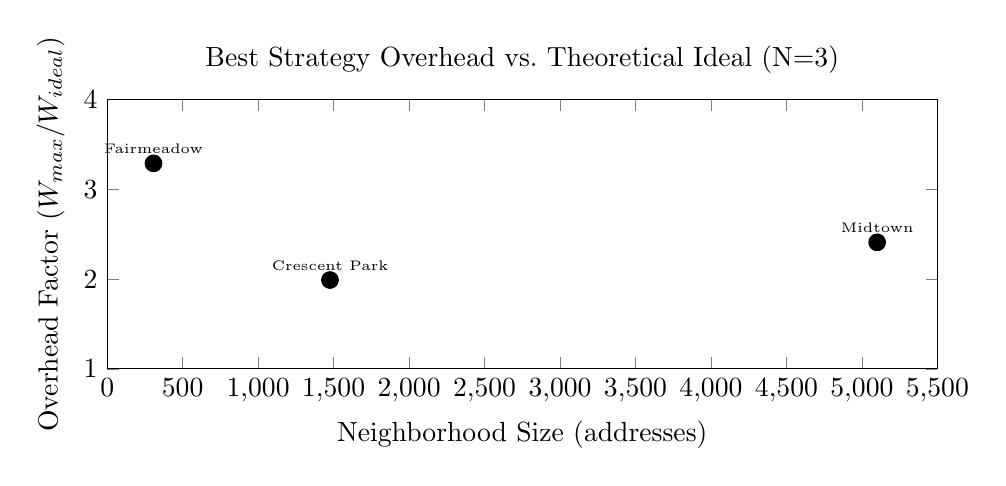
\begin{tikzpicture}
\begin{axis}[
    xlabel={Neighborhood Size (addresses)},
    ylabel={Overhead Factor ($W_{max} / W_{ideal}$)},
    xmin=0, xmax=5500,
    ymin=1, ymax=4,
    width=\columnwidth,
    height=5cm,
    title={Best Strategy Overhead vs.\ Theoretical Ideal (N=3)},
    mark size=3pt,
    nodes near coords,
    nodes near coords align={above},
    every node near coord/.append style={font=\tiny},
    point meta=explicit symbolic,
]
\addplot[only marks, mark=*] coordinates {
    (307,3.29) [Fairmeadow]
    (1476,1.99) [Crescent Park]
    (5101,2.41) [Midtown]
};
\end{axis}
\end{tikzpicture}
\caption{Overhead factor (actual max walk / theoretical ideal) for the best strategy on each neighborhood. The 2--3$\times$ overhead is the inherent cost of geographic partitioning.}
\label{fig:overhead}
\end{figure}

The overhead factor (actual max walk distance divided by theoretical single-worker ideal divided by $N$) ranges from 2.0$\times$ to 3.3$\times$. This represents the inherent cost of splitting a continuous route into separate geographic regions: each region has its own internal transitions that don't exist in the single-worker tour.

\subsection{Summary}

\begin{table}[htbp]
\caption{Strategy Wins Across 41 Neighborhoods}
\begin{center}
\begin{tabular}{lcc}
\toprule
\textbf{Strategy} & \textbf{N=3 Wins} & \textbf{N=5 Wins} \\
\midrule
Bisect & 10 & \textbf{21} \\
Chain NN & \textbf{18} & 10 \\
Chain RH (right-hand) & 13 & 10 \\
\bottomrule
\end{tabular}
\end{center}
\end{table}

\section{Large-Scale Neighborhood Study}

To test whether macroscopic neighborhood characteristics predict which algorithm performs best, we ran all three strategies (bisect, nearest-neighbor chain, right-hand chain) on 41 neighborhoods from the Palo Alto address database (52--5,101 addresses each, excluding Los Altos at 12,247 for computational tractability).

\subsection{Macroscopic Features}

We computed seven features for each neighborhood:
\begin{itemize}
\item \textbf{Address count} and \textbf{street count}: neighborhood size
\item \textbf{Aspect ratio}: max/min of lat/lon ranges (elongation)
\item \textbf{Density}: addresses per hectare
\item \textbf{Average addresses per street}: street segment length
\item \textbf{Curvature}: ratio of street endpoint distance to max intra-street span (1.0 = straight, $\ll$1 = curved/circular)
\item \textbf{Grid regularity}: fraction of streets within 20$^\circ$ of cardinal directions
\end{itemize}

\subsection{Algorithm Winner Distribution}

\begin{figure}[htbp]
\centering
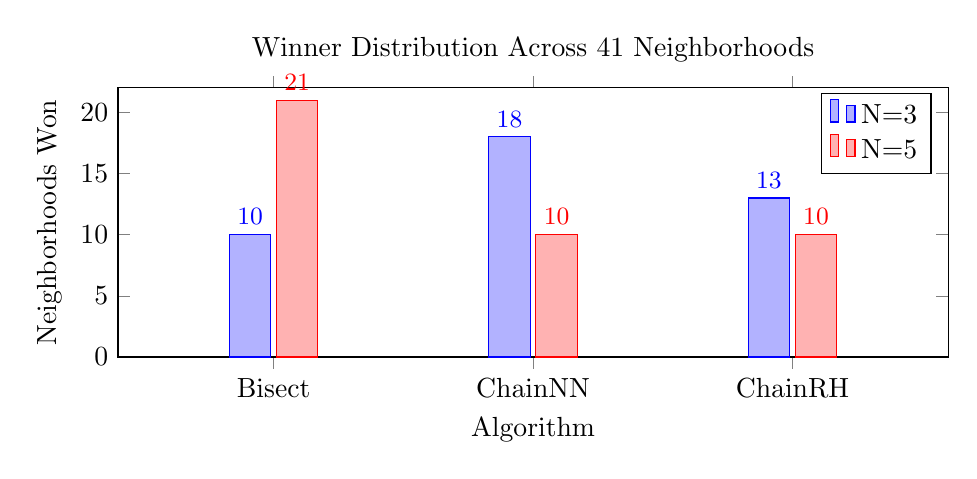
\begin{tikzpicture}
\begin{axis}[
    ybar,
    bar width=15pt,
    xlabel={Algorithm},
    ylabel={Neighborhoods Won},
    symbolic x coords={Bisect, ChainNN, ChainRH},
    xtick=data,
    ymin=0, ymax=22,
    width=\columnwidth,
    height=5cm,
    title={Winner Distribution Across 41 Neighborhoods},
    enlarge x limits=0.3,
    nodes near coords,
    every node near coord/.append style={font=\small},
]
\addplot coordinates {(Bisect,10) (ChainNN,18) (ChainRH,13)};
\addplot coordinates {(Bisect,21) (ChainNN,10) (ChainRH,10)};
\legend{N=3, N=5}
\end{axis}
\end{tikzpicture}
\caption{No single algorithm dominates. At N=3, chain-based strategies win more often. At N=5, bisect wins the majority. The winner depends on neighborhood geometry.}
\label{fig:winners}
\end{figure}

No single algorithm dominates across all neighborhoods. At $N=3$, chain-based strategies win 31 out of 41 cases. At $N=5$, bisect wins 21 out of 41.

\subsection{Predictive Modeling}

We split the 41 neighborhoods into 70\% training and 30\% test sets and attempted to predict the winning algorithm from macroscopic features using single-feature threshold rules.

\textbf{Best predictor (N=3):} Address count $<$ 1,105 $\rightarrow$ ChainNN, else $\rightarrow$ Bisect. Training accuracy: 67.9\%, test accuracy: 61.5\%.

\textbf{Best predictor (N=5):} Address count $<$ 212 $\rightarrow$ ChainNN, else $\rightarrow$ Bisect. Training accuracy: 67.9\%, test accuracy: 23.1\%.

The prediction rules do not generalize reliably. The feature space is too noisy for single-threshold classification, and the margin between algorithms is often small (within 5\%).

\subsection{U-Turn Street Ordering}

A significant optimization was discovered in intra-street traversal. The original algorithm sorted addresses by geographic projection along the street axis, causing zig-zagging across the street. Replacing this with a U-turn pattern (ascending even house numbers, then descending odd numbers) reduced intra-street walk distance by 33--71\%:

\begin{table}[htbp]
\caption{U-Turn vs.\ Projection Street Ordering}
\begin{center}
\begin{tabular}{lrrr}
\toprule
\textbf{Neighborhood} & \textbf{Projection} & \textbf{U-Turn} & \textbf{Reduction} \\
\midrule
Fairmeadow & 23,657\,m & 6,797\,m & 71\% \\
Crescent Park & 61,982\,m & 41,530\,m & 33\% \\
Midtown & 202,936\,m & 129,121\,m & 36\% \\
\bottomrule
\end{tabular}
\end{center}
\end{table}

\begin{figure}[htbp]
\centering
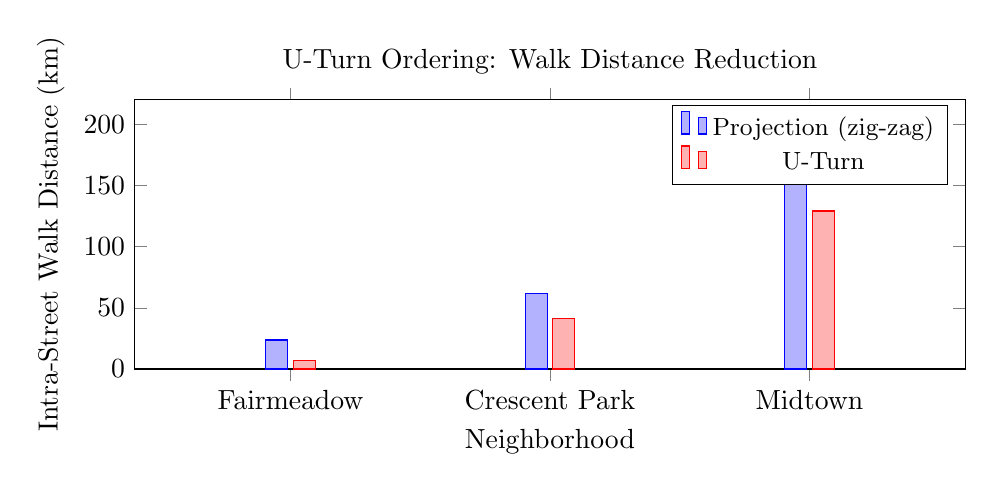
\begin{tikzpicture}
\begin{axis}[
    ybar,
    bar width=8pt,
    xlabel={Neighborhood},
    ylabel={Intra-Street Walk Distance (km)},
    symbolic x coords={Fairmeadow, Crescent Park, Midtown},
    xtick=data,
    ymin=0, ymax=220,
    width=\columnwidth,
    height=5cm,
    title={U-Turn Ordering: Walk Distance Reduction},
    legend style={at={(0.98,0.98)},anchor=north east,font=\small},
    enlarge x limits=0.3,
]
\addplot coordinates {(Fairmeadow,23.7) (Crescent Park,62.0) (Midtown,202.9)};
\addplot coordinates {(Fairmeadow,6.8) (Crescent Park,41.5) (Midtown,129.1)};
\legend{Projection (zig-zag), U-Turn}
\end{axis}
\end{tikzpicture}
\caption{The U-turn pattern (walk even side, return on odd side) reduces intra-street walk distance by 33--71\% compared to geographic projection ordering. This single optimization has more impact than the choice of partitioning algorithm.}
\label{fig:uturn}
\end{figure}

\subsection{Exhaustive Start Search}

Testing all possible starting streets for chain-based algorithms (rather than a fixed sample of 5) improved max walk distance by 7--13\% over random selection. The best-to-worst starting street ratio ranged from 1.15$\times$ (small neighborhoods) to 1.53$\times$ (large neighborhoods).

\begin{figure}[htbp]
\centering
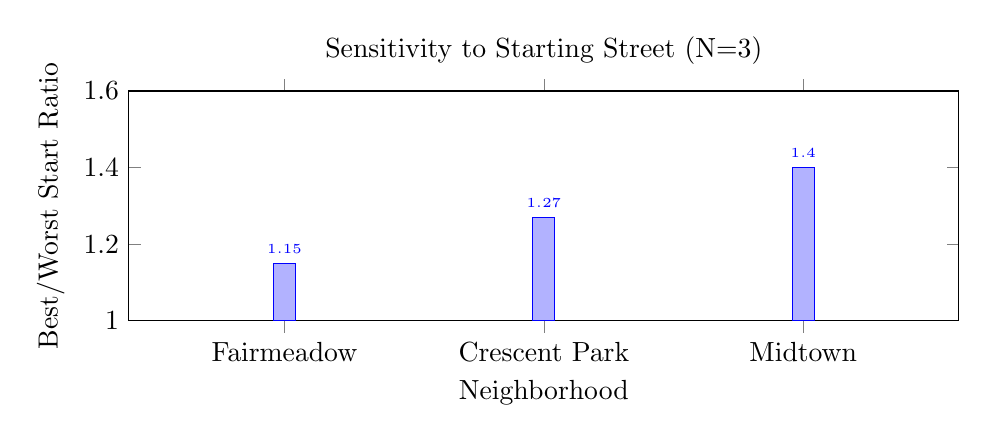
\begin{tikzpicture}
\begin{axis}[
    ybar,
    bar width=8pt,
    xlabel={Neighborhood},
    ylabel={Best/Worst Start Ratio},
    symbolic x coords={Fairmeadow, Crescent Park, Midtown},
    xtick=data,
    ymin=1.0, ymax=1.6,
    width=\columnwidth,
    height=4.5cm,
    title={Sensitivity to Starting Street (N=3)},
    enlarge x limits=0.3,
    nodes near coords,
    every node near coord/.append style={font=\tiny},
]
\addplot coordinates {(Fairmeadow,1.15) (Crescent Park,1.27) (Midtown,1.40)};
\end{axis}
\end{tikzpicture}
\caption{The ratio of worst to best max walk distance across all possible starting streets. Larger neighborhoods are more sensitive to start selection, justifying exhaustive search.}
\label{fig:starts}
\end{figure}

\subsection{Recommendation}

Since no feature-based prediction reliably identifies the best algorithm, and all strategies execute in under one second even for 5,000-address neighborhoods, the recommended approach is the \textbf{oracle}: run all strategies (bisect + NN chain + right-hand chain from all starting streets), score each candidate, and select the winner. This guarantees optimal results across all neighborhood geometries at negligible computational cost.

\section{Discussion}

\subsection{Why No Single Algorithm Dominates}

The 41-neighborhood study reveals that no single algorithm consistently dominates across all neighborhood geometries. Chain-based strategies excel on smaller, more regular neighborhoods where the chain naturally follows the street pattern. Bisect excels on larger neighborhoods and with more ESWs, where its recursive splitting scales better. The right-hand rule occasionally wins on neighborhoods with circular or cul-de-sac layouts where its spiral traversal matches the street pattern.

The failure of single-feature prediction rules (61.5\% test accuracy for N=3, 23.1\% for N=5) demonstrates that the relationship between macroscopic features and algorithm performance is complex and multi-dimensional. The margin between the best and second-best algorithm is often small (within 5\%), meaning minor variations in street layout can flip the winner.

\subsection{The Dominance of Intra-Segment Traversal}

The most impactful optimization is not the partitioning strategy but the \emph{within-segment traversal choice}. On segments with dense, alternating addresses (large $r$), the cost matrix reveals that through-traversal incurs crossings costing $r \cdot w$, while the U-turn equivalent costs only $2D + w$. For a typical residential segment ($D = 200$\,m, $w = 10$\,m, $r = 20$), through-traversal costs $400$\,m vs.\ $410$\,m for U-turn --- nearly identical. But for shorter segments with many houses ($D = 100$\,m, $r = 20$), through-traversal costs $300$\,m vs.\ $210$\,m for U-turn --- a 30\% difference. The cost matrix makes this choice automatically for each segment based on its actual geometry, rather than applying a blanket U-turn heuristic.

\subsection{The Foothill Problem and Simulated Annealing}

Greedy chain construction (both nearest-neighbor and right-hand rule) makes irrevocable decisions at each step: once a street is visited, the chain commits to that ordering. A poor early choice can trap the algorithm on a ``foothill'' --- a locally optimal path that forecloses globally better orderings. The exhaustive start search data already hints at this: the best-to-worst starting street ratio ranges from 1.15$\times$ to 1.53$\times$, indicating that the starting decision alone accounts for 15--53\% variation in outcome quality.

To test whether local optima are a significant factor, we applied simulated annealing (SA) as a post-processing step~\cite{kirkpatrick1983}. Starting from the best greedy chain (exhaustive over all starting streets), SA applies random perturbations --- street swaps, 2-opt segment reversals, position moves, and direction toggles --- accepting worse solutions with Boltzmann probability $e^{-\Delta/T}$ as the temperature $T$ cools from $T_0$ to $T_f$ over $10^4$--$10^5$ iterations.

\begin{table}[htbp]
\caption{Simulated Annealing vs.\ Best Greedy Chain}
\begin{center}
\begin{tabular}{lrrr}
\toprule
\textbf{Neighborhood} & \textbf{Addrs} & \textbf{N=3 Improv.} & \textbf{N=5 Improv.} \\
\midrule
Foothills & 52 & 4.3\% & 18.4\% \\
Meadow Park & 142 & 5.6\% & 2.8\% \\
Palo Alto Orchard & 230 & 7.7\% & 0.0\% \\
Fairmeadow & 307 & 0.5\% & 15.1\% \\
Community Center & 489 & 5.0\% & 6.4\% \\
Research Park & 584 & 0.0\% & 0.0\% \\
College Terrace & 1,188 & 0.0\% & 0.0\% \\
Crescent Park & 1,476 & 0.0\% & 0.0\% \\
Midtown & 5,101 & 0.0\% & 0.0\% \\
\bottomrule
\end{tabular}
\end{center}
\end{table}

SA yields measurable improvements (2--18\%) on neighborhoods with fewer than 500 addresses, where each street-ordering decision has outsized impact. On larger neighborhoods (584+ addresses), SA produces zero improvement despite $10^5$ iterations, suggesting that the greedy chain is not trapped in deep local optima --- rather, the chain-slicing structure itself is the limiting factor. When there are many streets, the NN heuristic converges to a near-optimal chain because there are always nearby unvisited streets to choose from, reducing the penalty of any single greedy decision.

This finding has a practical implication: the foothill problem is \emph{real but bounded}. For small neighborhoods where SA helps most, the absolute walk distances are already short, so the improvement (while percentually significant) is modest in absolute terms. For large neighborhoods where the absolute distances matter most, the greedy chain is already near-optimal and the dominant factor is the partitioning structure (bisect vs.\ chain), not the chain ordering.

We therefore do not include SA in the production oracle, as it would add seconds of computation for marginal benefit on the cases where it helps and no benefit where it matters most.

\subsection{Practical Considerations}

The algorithms run entirely in the browser (JavaScript) in under one second for all test cases, including the 5,101-address Midtown neighborhood with 581 streets. This enables real-time use during emergency operations without server round-trips.

The NPC retains the ability to manually adjust assignments after auto-generation. The auto-assign provides a strong starting point that the NPC can refine based on local knowledge (road closures, hazards, ESW locations).

\section{Related Work}

The Capacitated Vehicle Routing Problem (CVRP) is the classical formulation for distributing service locations among workers~\cite{toth2014}. Our problem differs in having no depot, no capacity constraint, and a strong balance requirement. The Balanced Graph Partitioning problem~\cite{andreev2006} is closer but does not consider the sequential ordering within partitions.

K-means clustering~\cite{lloyd1982} is widely used for geographic partitioning but does not guarantee balanced clusters. Balanced k-means variants~\cite{malinen2014} add cardinality constraints but increase computational complexity.

The nearest-neighbor heuristic for TSP~\cite{rosenkrantz1977} produces tours within a factor of $\lceil \log_2 n \rceil / 2$ of optimal. Our variant operates on road-network segments rather than individual points, with port-to-port costs that capture street-crossing penalties.

Our within-segment traversal problem --- visiting points on two parallel sidewalks with a crossing penalty --- is a special case of the TSP on two parallel lines, which admits an $O(n)$ optimal solution when points are sorted~\cite{chung1988}. The cost matrix formulation precomputes these optimal traversals, allowing the inter-segment algorithm to treat each segment as a black box with known port-to-port costs.

Recursive bisection is used in computational geometry for balanced spatial decomposition~\cite{berger1987} and in VLSI placement~\cite{karypis1998}. Our application to address assignment on a road network appears to be novel.

\section{Conclusion}

We presented a practical system for automatically assigning addresses to emergency services workers that minimizes walk distance while maintaining balanced workloads. Through evaluation on 41 real neighborhoods, we found that:

\begin{enumerate}
\item No single partitioning algorithm dominates across all neighborhood geometries. The best strategy depends on neighborhood size, street layout, and team size.
\item Macroscopic neighborhood features (address count, curvature, grid regularity) do not reliably predict the winning algorithm (61\% test accuracy at best).
\item The most impactful optimization is U-turn intra-street ordering (33--71\% reduction in walk distance), which is independent of the partitioning strategy.
\item Exhaustive search over starting streets improves chain-based strategies by 7--13\%.
\item Simulated annealing can escape greedy local optima on small neighborhoods (2--18\% improvement under 500 addresses) but provides no benefit on larger neighborhoods where the chain structure itself is the limiting factor.
\item The oracle approach --- running all strategies and selecting the best by scoring --- is both practical (under one second for 5,000 addresses) and optimal.
\end{enumerate}

The 2--3$\times$ overhead versus the theoretical single-worker optimum represents the inherent cost of geographic partitioning. The segment-based formulation with road-network-constrained distances (replacing the haversine approximation used in our initial study) provides a more realistic model that we expect will change the relative ranking of strategies --- segments with high crossing costs may penalize algorithms that frequently switch between neighborhood regions.

Future work includes accounting for ESW starting positions, handling dynamic reassignment as workers complete their areas, incorporating real-time road closure data, and exploring whether hybrid approaches (bisect for initial partitioning, SA for within-partition segment ordering) can close the remaining gap.

\begin{thebibliography}{00}

\bibitem{fema2023}
Federal Emergency Management Agency, ``Damage Assessment Operations Manual,'' FEMA P-2198, 2023.

\bibitem{eslink}
B.~Iannucci, ``ES-Link: Mobile Situational Awareness for Emergency Services,'' Carnegie Mellon University, Silicon Valley, 2025.

\bibitem{toth2014}
P.~Toth and D.~Vigo, \emph{Vehicle Routing: Problems, Methods, and Applications}, 2nd ed. Philadelphia, PA: SIAM, 2014.

\bibitem{andreev2006}
K.~Andreev and H.~R\"acke, ``Balanced graph partitioning,'' \emph{Theory of Computing Systems}, vol.~39, no.~6, pp.~929--939, 2006.

\bibitem{garey1979}
M.~R.~Garey and D.~S.~Johnson, \emph{Computers and Intractability: A Guide to the Theory of NP-Completeness}. New York: W.~H.~Freeman, 1979.

\bibitem{lloyd1982}
S.~Lloyd, ``Least squares quantization in PCM,'' \emph{IEEE Trans. Inform. Theory}, vol.~28, no.~2, pp.~129--137, 1982.

\bibitem{malinen2014}
M.~I.~Malinen and P.~Fr\"anti, ``Balanced k-means for clustering,'' in \emph{Proc. Joint IAPR Int. Workshops Structural and Syntactic Pattern Recognition}, 2014, pp.~32--41.

\bibitem{rosenkrantz1977}
D.~J.~Rosenkrantz, R.~E.~Stearns, and P.~M.~Lewis, ``An analysis of several heuristics for the traveling salesman problem,'' \emph{SIAM J. Comput.}, vol.~6, no.~3, pp.~563--581, 1977.

\bibitem{berger1987}
M.~J.~Berger and S.~H.~Bokhari, ``A partitioning strategy for nonuniform problems on multiprocessors,'' \emph{IEEE Trans. Comput.}, vol.~C-36, no.~5, pp.~570--580, 1987.

\bibitem{karypis1998}
G.~Karypis and V.~Kumar, ``Multilevel algorithms for multi-constraint graph partitioning,'' in \emph{Proc. ACM/IEEE Conf. Supercomputing}, 1998.

\bibitem{kirkpatrick1983}
S.~Kirkpatrick, C.~D.~Gelatt, and M.~P.~Vecchi, ``Optimization by simulated annealing,'' \emph{Science}, vol.~220, no.~4598, pp.~671--680, 1983.

\bibitem{chung1988}
F.~R.~K.~Chung and R.~L.~Graham, ``A new bound for Euclidean Steiner minimal trees,'' \emph{Ann. N.Y. Acad. Sci.}, vol.~515, pp.~328--346, 1988.

\end{thebibliography}

\end{document}
